\section{Micro Processing Unit}

Denne sektion kommer omkring de forskellige moduler, som mikroprocessoren håndterer, samt hvilket styresystem der anvendes.

\subsection{Operativ System}
Når der skal skiftes mellem flere tasks som en processor skal udføre, er det vigtigt at kunne skifte mellem dem på en fornuftig måde; Dette udføres ved hjælp af en schedulerings algoritme. Når der skal implementeres en schedulerings algoritme skal det overvejes hvorvidt det er nødvendigt at lave én designet specielt til projektet, eller om der en en eksisterende der er i stand til at udføre opgaven tilstrækkeligt. I dette project har vi to muligheder til rådighed: FreeRTOS\cite{FreeRTOSorg} og en Run To Complete Scheduler (RTCS).

\subsubsection{FreeRTOS}

FreeRTOS \cite{FreeRTOSorg} er et realtids operativsystem (RTOS), der er en standard løsning som bliver brugt i en mikroprocessor. FreeRTOS giver os muligheden for at bruge preemptiv skedulering, hvilket vil sige at CPU'en kan springe imellem tasks, og hoppe ud af dem efter behov. Dette bliver styret ud fra hvilken prioritet task'en har, eller om der en anden task, der får et interrupt, den skal holde øje med.
\\
Udover dette har freeRTOS også mange andre funktioner dette projekt kan udnytte. Der er mulighed for at oprette køer, som vil blive nævnt som queues. Disse queues kan man sende events og data til ved hjælp af en funktion der hedder xQueueSend. 
\\
FreeRTOS kan lave semaforer, som gør det muligt at flere tasks skal kunne tilgå disse queues, disse semaforer gør at kun en task der har adgang til queue'en indtil semaforen bliver frigjort igen. For at ungå at styre systemet ikke bliver fastlåst i denne semafor for evigt indsættes der en tid, den kan være inde i semaforen.
\\
Queues og semaforer bliver oprettet ef xQueueHandle og xSemaphoreHandle. Hvorefter de bliver kreeret ved hjælp af xQueueCreate og xSemaphoreCreateMutex. For at bruge xQueueCreate skal der også bruges størrelse af queue'en og hvilken parameter den skal indeholde.
\\
FreeRTOS tilbyder også et Shared State Memory (SSM), dette gør det muligt at CPU'en kan hoppe imellem de forskellige tasks. F.eks. hvis der kommer et event på UART, som kunne være "STOP\textunderscore EVENT". Dette event gør, at den med det samme går over til den case hvor eventet er, og gør som der står, som i dette tilfælde er at bremse motoren.

\subsubsection{RTCS}

Run To Complete Scheduler (RTCS) er en anden måde at køre ens styresystem på. Den kører som en non preemtiv skedulering, hvilket vil sige at lige så snart CPU'en har forbindelse til en proces/task, så kan den ikke hoppe ud af denne proces/task. I dette system kan der også oprettes queue's.
\\
Den har mulighed for at oprette semaforer, som gør at det er kun en task som kan have adgang til queue'en. For at tilføje data til en queue skal funktionen put\textunderscore queue kaldes. Funktionen wait\textunderscore sem bruges til at tilføje en semafor til den specifikke queue.

\subsubsection{Valg af Operativsystem}

Efter vi har set på disse to valg muligheder kan vi se at RTCS vil være næmmere at få til at virker, fordi det ikke er så komplicert og har ikke lige så mange udvidelser. RTCS tilbyder dog ikke de samme sikkerhed udvidelser som freeRTOS gør. Den største begrundelse for at vi vælger at arbejde med freeRTOS over RTCS er, at den kører preemptiv skedulering. Dette gøre det muligt, hvis der kommer et vigtigt interrupt, at den kan tage CPU'en fra den proces den er i gang med, og flytte den over til den vigtigste proces.

\subsection{Tasks}

Der er blevet lavet et task diagram(se figur \ref{fig:task1}, \ref{fig:task2} og \ref{fig:task3}) her under udviklingen af programet til microcontrolleren. Kommunikation mellem tasks foregår gennem både queues og Shared State Memory. Shared state memory benyttes når der skal sendes data i form af ændring af variabler mellem tasks, mens queues benyttes til at sende beskeder i form af events eller data. Denne metode blev valgt fordi opstår situationer hvor flere tasks skal bruge de samme informationer, og deres eventuelle ændringer af dem påvirker de andre tasks, der skal have kendskab til samme variable.
\\
Af samme årsag benyttes der en semafor til at begrænse adgangen til disse, så der ikke opstår synkroniseringsfejl.
\\
Den centrale task er Menu'en. Denne styrer en menu, der har til opgave at give mulighed for manuelt at sætte variabler, såsom tid og position, samt at starte og stoppe vores kontrolsystem, og kommunikere tilbage gennem UART transmit. De tasks som er bygget op omkring denne kan ses i figur \ref{fig:task1}.
\\
Da der er flere forskellige tasks, der skal have adgang til de samme værdier der bliver sat af UART bliver værdierne, der tages gennem denne, sat i shared state memory, som det ses på figur \ref{fig:task2}.
\\
Display tasken holder selvsigende styr på hvad der skal vises, som den får besked om fra Menu'en. Denne får input fra keypad'en og drehimpulsgeberen, der dikterer hvad den skal give videre til LCD.
\\
Geber og Keypad tasksne holder styr på hver deres input, og sender resultaterne i en fælles indgangs kø til Menu'en.
\\
Control systemet tager med jævne mellemrum variabler fra Shared State Memory, og benytter disse til at opdatere det mål pan/tilt-systemet går efter. Den kommunikerer så frem og tilbage med SPI-task'en, som kommunikerer med vores FPGA. Task diagrammet for denne kan ses i figur \ref{fig:task3}.
\\
Årsagen til at dette layout er blevet valgt er at det vurderes at kontrolsystemet ikke skal være afhængig af input fra Menu'en, så det ikke er nødvendigt at benytte menuen til at give den nye koordinater. Ved at separerer den fra Menuen er det muligt for den at køre selvstændigt, uden at den yderligere skal checke en kø for nye koordinater hele tiden.

\begin{figure}[ht]
			\begin{center}
	\includegraphics[width=0.99\textwidth]{Billeder/Taskdiagram1.png}
			\end{center}
	\caption{Task diagrammet over de dele af systemet der centreres over menu'en. Der gives input til UI task'en som så videre giver information hvor der er brug for det, i dette tilfælde Display tasken, Shared State Memory og UART transmit.}
	\label{fig:task1}
\end{figure}

\begin{figure}[ht]
			\begin{center}
\includegraphics[width=0.99\textwidth]{Billeder/Taskdiagram2.png}
			\end{center}
	\caption{Task diagrammet over UART receive. Informationen gemmes i Shared State Memory.}
	\label{fig:task2}
\end{figure}

\begin{figure}[ht]
			\begin{center}
\includegraphics[width=0.99\textwidth]{Billeder/Taskdiagram3.png}
			\end{center}
	\caption{Task diagrammet over kontrol systemet. De værdier den skal bruge kommer fra SPI task'en og eller fra Shared State Memory.}
	\label{fig:task3}
\end{figure}

%\begin{figure}[!ht]
%\centering
%\begin{subfigure}[t]{0.3\textwidth}
%	\includegraphics[width=0.99\textwidth]{Billeder/Taskdiagram1.png}
%	\caption{Task diagrammet over de dele af systemet der centreres over menu'en. Der gives input til UI task'en som så videre %giver information hvor der er brug for det, i dette tilfælde Display tasken, Shared State Memory og UART transmit.}
%	\label{fig:task1}
%    \end{subfigure}
%    \begin{subfigure}[t]{0.3\textwidth}
%	\includegraphics[width=0.99\textwidth]{Billeder/Taskdiagram2.png}
%	\caption{Task diagrammet over UART receive. Informationen gemmes i Shared State Memory.}
%	\label{fig:task2}
%    \end{subfigure}
%    \begin{subfigure}[t]{0.3\textwidth}
%	\includegraphics[width=0.99\textwidth]{Billeder/Taskdiagram3.png}
%	\caption{Task diagrammet over kontrol systemet. De værdier den skal bruge kommer fra SPI task'en og eller fra Shared State Memory.}
%	\label{fig:task3}
%    \end{subfigure}
%\label{fig:taskdiagram}
%\caption{Vores task diagram tager udgangspunkt i en UI der sender besked til et display, hvilket benyttes til at vise en menu der kan bruges til at opdaterer diverse parametre og mål, hvilket så gives videre til det implementerede control system gennem Shared State Memory.}
%\end{figure}


\subsubsection{Menu}

Den centrale task i systemet er det menu styrede UI-system. Denne har primært til opgave at give brugeren mulighed for manuelt at justere, starte eller stoppe systemet, samt at vise vigtige oplysninger som eksempelvis nuværende position. Menuen styres med drehimpulsgeber og keypad'et, som begge lægger events ind i dens input kø. Den giver events videre til GUI tasken, som styrer de forskellige menuer og display funktioner.



\subsubsection{Universal Asynchronous Receiver/Transmitter}

UART står for universal asynchronous receiver/transmitter. Dette laver kommunikation mellem to enheder. UART transmitterer data i form af bytes og deler dem op i bits og sender dem. Modtager skal så kunne samle dem sammen igen til bytes for at læse det. Uart har en init() funktion som bliver kaldt en gang hvor alle registre bliver sat op som, f.eks. send og modtag. Der bliver også sat en baud rate, som skal være den samme for sender og modtager.
\\
For at sende data kalder vi funktion uart0\textunderscore putc som tager en karakter som input. Dette kan både være tal og bogstaver. Der er en funktion der hedder uart0\textunderscore rx\textunderscore rdy som venter på at den modtager noget.
\\
For at gøre det nemmere har vi lavet en lille protokol, som skal overholdes før microcontrolleren kan tyde det. I figur \ref{fig:UARTCMD} kan ses en liste over de forskellige commands. Et eks. på en UART kald kunne være \texttt{\char`\\}st1803 , som vil sætte tilt delen til 180,3 grader.

\begin{figure}[ht]
			\begin{center}
			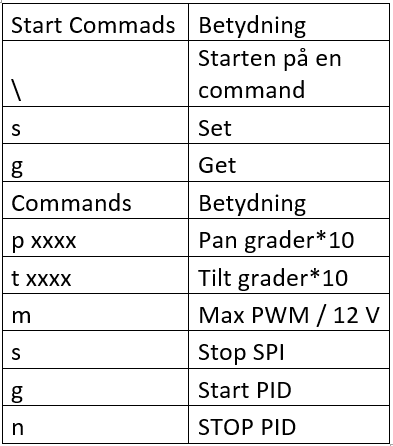
\includegraphics[scale=0.5]{Billeder/UARTCMD.png}
			\end{center}
			\caption{UART commands}
			\label{fig:UARTCMD}
\end{figure}

\subsubsection{Display}

Display task'en tager input fra Menu-task'en og bruger dem til at vælge fra en tabel over prædefinerede billeder, der så sendes til LCD task'en. Disse prædefinerede billeder kan så redigeres hvis der er brug for dette, hvilket er tilfældet hvis der skal vises en dynamisk værdi, som ved show-pan og show-tilt menu-mulighederne.

\subsubsection{LCD}

Den fysiske opsætning af LCD'et kan ses på figur \ref{fig:LCD}, og viser blandt andet at fire databen og R/W benet er forbundet til stel. Med denne opsætning kan man kun skrive til displayet ligesom man er tvunget til at bruge LCD'et i 4-bit mode. Hvis man havde mulighed for at læse fra displayet, kunne man holde øje med et busyflag, der fortæller om LCD'et er optaget, og på den måde sørge for at udnytte displayets tid bedst muligt. Når man kun kan skrive til displayet, er man tvunget til at vente en bestemt tid for at sikre sig at det er klar til at modtage ny data. Til de fleste formål er det dog ikke et problem, at man venter lidt længere end nødvendigt imellem kommandoer. I 4-bit mode kan der kun sendes en nibble ad gangen. For at sende data til displayet, skal dataen skrives ud på de fire databen, derefter flasher man E-benet så LCD'et kan latche og starte behandlingen. RS-benet styrer om den data, der sendes, skal tolkes som data eller en kommando. 

\begin{figure}[ht]
			\begin{center}
			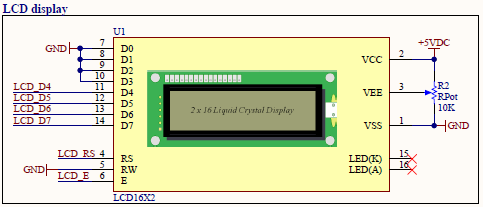
\includegraphics[scale=0.9]{Billeder/LCD.PNG}
			\end{center}
			\caption{LCD pinout}
			\label{fig:LCD}
\end{figure}

Selve LCD-task'en arbejder sammen med resten af systemet ved at afkode et særligt image-format (se figur \ref{fig:LCD_array}), så det vises korrekt på skærmen. Dette image bliver sendt fra display-task'en og indeholder oplysninger om, hvilke karakterer, hvis nogen, der skal skrives til alle 32 synlige adresser på displayet. Udover de 32 karakterer, er der også fire kontrolfelter, som fortæller task'en, hvor cursoren skal placeres efter karaktererne er skrevet ud; om cursoren skal blinke eller bare highlighte nuværende adresse med en streg under karakteren. Det sidste felt bliver sat til at vise adressen, hvor næste karakter skal skrives, når alle 32 karakterer er blevet skrevet første gang. På den måde kan LCD-tasken afgøre om den skal skrive et helt image fra starten, eller bare tilføje en ny karakter til et image der allerede er vist på displayet. Med dette setup kan LCD-tasken finde ud af hvilken ny karakter, der skal tilføjes ud fra den første kontrol-bit, samt hvor cursoren skal placeres efter den er skrevet - hvis den næste adresse, der skal skrives på, er mere end en plads væk, skal cursoren flyttes aktivt. Manipuleringen af images og kontrol-bits foregår i display-task'en - LCD-task'en afkoder bare images, når de bliver tilføjet til dens input-kø.


\begin{figure}[ht]
			\begin{center}
			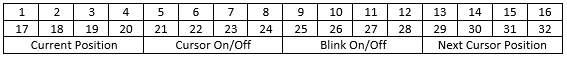
\includegraphics[scale=0.9]{Billeder/LCD_Array.PNG}
			\end{center}
			\caption{LCD Image-format er et array af 36 8-bits størrelser. De første 32 pladser i arrayet repræsenterer de synlige adresser på displayet - de sidste 4 er kontrol-bits.}
			\label{fig:LCD_array}
\end{figure}

\subsubsection{Keypad}

Det udleverede Kit har et tilhørende keypad med 12 knapper fra 0 til 9, samt * og \#. Dette keypad virker som knapper, det er derfor nødvendigt at definere hvad de forskellige knapper skal gøre. For at gøre det simpelt bliver hver knap sat til dens tilsvarende ascii-karakter. Figur \ref{fig:Keypadpins} viser hvordan dens pins er tilsluttet.
\begin{figure}[ht]
	\begin{center}
		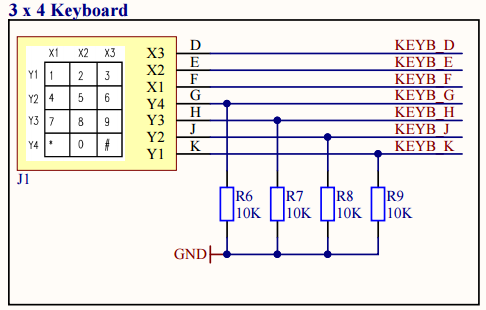
\includegraphics[scale=0.7]{Billeder/Keypadpins.PNG}
	\end{center}
\caption{Keypad pinout}
\label{fig:Keypadpins}
\end{figure}
Den har to porte til knyttet som er PORT A og PORT E. Det betyder at vi kan læse på port E hvis GPIO pinden på port A er aktiv.
\begin{figure}[ht]
	\begin{center}
		\includegraphics[scale=0.7]{Billeder/Keypad.PNG}
	\end{center}
\caption{Giver de fysiske placeringer et tal, som svare et en placering i et array, så som at 1 for placering 24}
\label{fig:Keypad}
\end{figure}


På figur \ref{fig:Keypad} kan vi se at vi har givet de forskellige knapper unikke værdier. Dette gøres fordi vi har et array som indeholder alle fysiske placeringer på keypad’et, som bliver placeret i den plads i array som kan ses på figur \ref{fig:Keypad} . For at finde en karakter kigger vi først på alle X værdier (port A) igennem og ser om en Y værdi (port E) er aktiv og ud fra hvilken X og Y værdi kan vi finde ud fra hvilket plads i arrayet, som blivet defineret i figur \ref{fig:Keypad}
\\
Dette keypad kan blive brugt til at sende data eller manuelt indsætte nogle værdier imens programmet kører.



\subsubsection{DrehImpulsGeber}

Ved at skrue på drehimpulsgeber kan man inkrementere eller dekrementere en variabel eller sende et event.
Drehimpulsgeberen er en roterende knap som også kan trykkes ned.\\
Drehimpulsgeberen kan sende 30 pulser per rotation.

\begin{figure}[ht]
			\begin{center}
			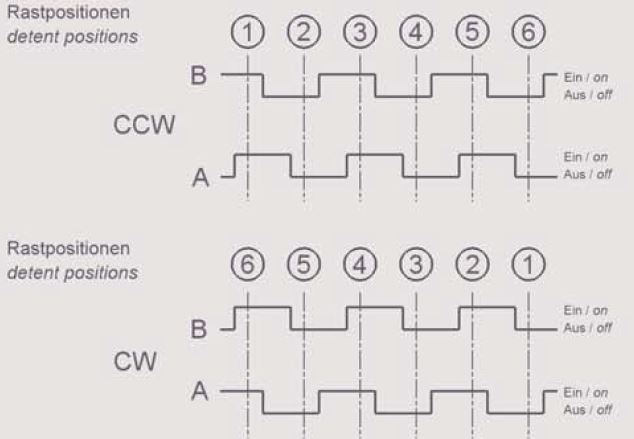
\includegraphics[scale=0.40]{Billeder/DrehImpulsGeber_events.jpg}
			\end{center}
			\caption{Drehimpulsgeber states}
			\label{fig:Impulsgeber}
		\end{figure}

For at finde ud af hvilken retning der bliver skruet på impulsgeberen, kigges der på de tidligere states af switchen.
eksempelvist hvis der kigges på figur \ref{fig:Impulsgeber} ses det at værdien af B ved henholdsvis en rising eller falling edge på A afhænger af retningen drehimpulsgeberen drejer. Dette bruges til at bestemme hvilket input der skal registeres.


\subsection{Serial Peripheral Interface}
\label{subsec:SPI}

Microcontrolleren (TM4C123GH6PM) der blev udleveret dette semester  indeholder 4 SSI (Synchronous Serial Interface) da disse 4 interfaces alle er ens, med undtagelse af deres pins, er SSI0 blevet valgt som interface, dvs. port A pin 2 er til SSI0Clk (modulets clock), pin 3 er SSI0Fss (frame signalet), pin 4 er SSI0Rx (modtagelse) og pin 5 er SSI0Tx (afsendelse).

Til SSI modulet er der 3 forskellige data formater:

\begin{itemize}
	\item Texas Instruments Synchronous Serial
		\begin{figure}[ht]
			\begin{center}
			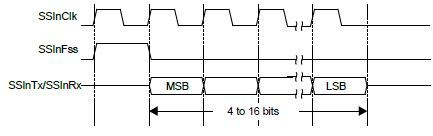
\includegraphics[scale=1]{Billeder/TI_Synchronous_Serial_Frame_Format.jpg}
			\end{center}
			\caption{TI Synchronous Serial Frame Format (Single transfer)}
			\label{fig:TIFrameFormat}
		\end{figure}

	\item Freescale SPI
		\begin{figure}[ht]
			\begin{center}
			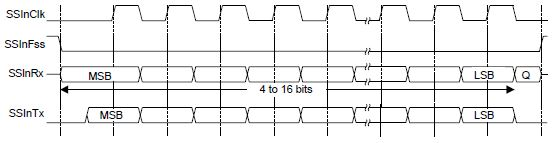
\includegraphics[scale=1]{Billeder/FS_Frame_Format.jpg}
			\end{center}
			\caption{FreeScale Frame Format (Single Transfer)}
			\label{fig:FSFrameFormat}
		\end{figure}
		  
	\item Microwire
		\begin{figure}[ht]
			\begin{center}
			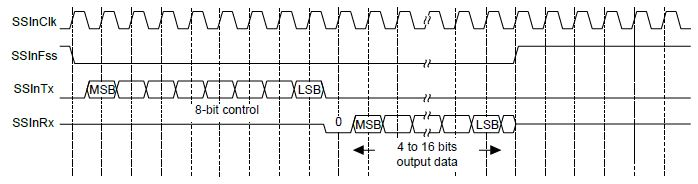
\includegraphics[scale=0.8]{Billeder/MW_Frame_format.jpg}
			\end{center}
			\caption{Micro Wire Frame Format (Single Transfer)}
			\label{fig:MWFrameFormat}
		\end{figure}
\end{itemize}

Da Freescale er den eneste SPI iblandt de tre SSI moduler er det den, der blev valgt.

		\begin{figure}[ht]
			\begin{center}
			\includegraphics[scale=0.8]{Billeder/Spi_Setup.jpg}
			\end{center}
			\label{fig:SPI_Setup}
			\caption{Setup af Freescale SPI}
		\end{figure}

For at lave et Freescale setup skal SSI modulet deaktiveres, og så kan microcontrolleren sættes som master ved at skrive nul til control registret.
Derefter skal clock configurations registret sættes til 0 så system clocken bruges.
Da der ønskes en 2 Mbps clock bruges følgende ligning

\begin{align*}
2*10^6 bps &= \dfrac{16*10^6 Hz}{CPSDVSR * (1 + 0)}\\
CPSDVSR &= \dfrac{16*10^6 Hz}{2*10^6 bps}\\
CPSDVSR &= 8
\end{align*}

Så sættes kontrol registret for SSI0 til 0xF da bit 3:0 angiver data størrelse, 0xF er så 16-bit data. Samtidig bliver Freescale SPI sat op, da bit 4 og 5 bestemmer frame formatet, og hvis de begge er lave betyder det at Freescale er valgt. 
og igen sættes bit 1 i kontrol registret for SSI1 til høj så SSI'en er aktiveret.

\subsection{PID-Controller}

PID-controllerens opgave består i at beregne sig frem til et passende PWM-signal, til at regulere motoren med, ud fra forskellen imellem motorens ønskede og faktiske position. Dette PWM-signal skal drive fejlen i 0 på en måde, der opfylder projektets designmål. Beregningen er styret af de tre konstanter $K_{P}$, $K_{I}$ og $K_{D}$, som man, igennem en analyse af systemets opførsel, beregner sig frem til. Denne analyse antager et ideelt system, hvor man hele tiden med uendeligt små tidsintervaller kan justere controllerens output. Det er ikke muligt at implementere en controller i den form, så der vil være en forskel på den programmerede og den modellerede controllers opførsel.


\subsubsection{Basal Virkemåde}

Selve udregningen af outputtet sker ved, at controlleren med jævne mellemrum kigger på setpointet for en motor, og sammenligner det med motorens faktiske position. Dette giver en fejlværdi som der løbende holdes øje med. 
\begin{itemize}
\item For at finde proportionaltermet ganges konstanten $K_{P}$ på fejlværdien
\item For at finde integraltermet ganges konstanten $K_{I}$ på en løbende summering af arealet under fejlen. Dette areal findes ved at gange $dt$ på fejlen, og så lægge det til hver gang udregningen køres igennem. På figur \ref{fig:Riemann} kan man se, hvordan integralet hele tiden vokser, så længe en fejl er til stede.
\item For at finde differentialtermet ganges konstanten $K_{D}$ på forskellen imellem den nuværende fejl og den forrige fejl delt med dt. Det svarer til at beregne $\Delta e/\Delta t$.
\end{itemize}

\begin{figure}[ht]
	\begin{center}
	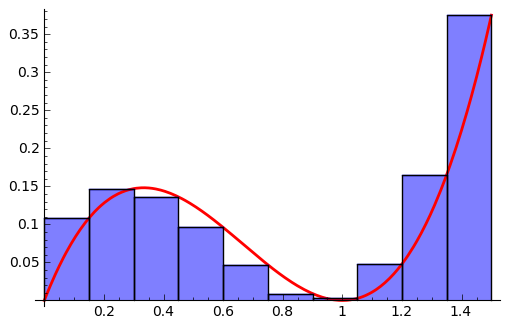
\includegraphics[scale=0.8]{Billeder/RiemannSum.png}
	\end{center}		
	\caption{Her ses en visualisering af det løbende integral der udregnes i starten af hver sample-periode. Arealet dækket af alle de blå bjælker viser størrelsen af integralet, og den røde kurve viser hvordan fejlen ændrer sig over tid.}
	\label{fig:Riemann}
\end{figure}

Når de tre termer er fundet, summeres de for at finde det endelige output fra udregningen. Dette output er i sig selv ikke brugbart til at finde en duty cycle som motoren skal reguleres med. Man er nødt til at definere et interval som outputtet kan operere indenfor. På den måde kan man, ved at finde ud af hvor outputtet befinder sig i intervallet, mappe denne position til en duty cycle mellem 0 og 255. På figur \ref{fig:Mapping} kan man se en visualisering af denne mapping. Hvis outputtet er negativt betyder det at retningen skal ændres på motoren, men det ændrer ikke noget på hvilken duty cycle, der skal sendes i sidste ende.

\begin{wrapfigure}{R}{0.5\textwidth}
	\begin{center}
	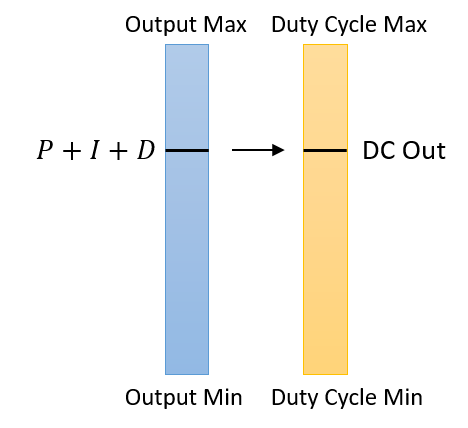
\includegraphics[scale=0.8]{Billeder/Mapping.png}
	\end{center}		
	\caption{Her ses hvordan PID-outputtet mappes til en tilsvarende duty cycle}
	\label{fig:Mapping}	
\end{wrapfigure}
\paragraph{Duty Cycle}

Det har en ret stor betydning hvilke duty cycles man kan sætte som output. Med duty cycles under 15 $\%$ kan man, for eksempel næsten ikke slæbe systemet rundt, og når man over 75 $\%$ kan systemet justere så voldsomt at selve platformen, rammerne er monteret på, begynder at flytte sig rundt på bordet. Af den grund blev der sat et interval mellem 15 $\%$ og 39 $\%$ som controlleren kunne justere indenfor. For at forhindre systemet i at oscillere omkring set point'et med en duty cycle på 15 $\%$ låses motoren, når fejlen er 0.

\paragraph{Skalering}

Et problem ved at bruge FreeRTOS som platform er, at det ikke er muligt at regne med floating point tal. Microcontrolleren kan fint arbejde med dem, da den har et floating point unit, men port mappet til FreeRTOS er lavet til en processor der ikke har en. Det giver problemer når FreeRTOS laver kontekst skift. Den kan ikke finde ud af at gemme floats i memory, når der skiftes imellem tasks. Så hvis der benyttes floats, så trapper styresystemet til et fault interrupt.

Af den grund er alle udregninger nødt til at foregå på heltal. For at kunne slippe afsted med det, er man nødt til at skalere operanderne i udregningerne, da der tit er tale om kommatal i en eller anden størrelsesorden. Den elegante og mest effektive løsning fås ved at bruge \textit{fixed point} aritmetik. Det kan dog være lidt svært at tyde tallene, når man læser koden, da de bliver konverteret til en størrelse der ikke, ved første øjekast, har nogen relation til det oprindelige tal. En simplere løsning i samme boldgade, som vi også endte med at bruge, er at skalere tallene med størrelsesordner af faktor 10. Det gør tallene ret store, men i kraft af at microcontrolleren arbejder med 32 bits ad gangen, er der ret højt til loftet. Det er også lettere for normale mennesker at arbejde med tal i base 10.

Det er vigtigt at sørge for at alle termerne bliver skaleret lige meget, så forholdet imellem termerne ikke ændres. De to ting der er nødvendige at skalere er $dt$ og gainet til controlleren, da de begge er i størrelsesorden $10^{-3}$. Det er så her man skal holde tungen lige i munden, for P-termet bliver kun påvirket af gainet og både I- og D-termet bliver påvirket af gain og $dt$, men D-termet bliver påvirket af $dt$-skaleringen modsat i forhold til I-termet. Så det vil sige at man, med en skaleringsfaktor på $10^4$, ender med et P-term skaleret med $10^4$, et I-term skaleret med $10^8$ og et D-term skaleret med $10^0$. Det skal der selvfølgelig justeres for, så outputtet giver mening.

\paragraph{Integral Windup}

Et problem med PID-controlleren er integral windup. Integral windup er, når arealet under fejlen vokser sig så stort at I-termet kommer til at dominere outputtet. Det er et stort problem for især langsomme systemer, som bruger lang tid på at drive fejlen i 0. Så længe der er en fejl til stede, vil integralet vokse sig større. Det kan blive så stort at systemet er nødt til at tilbringe lang tid med en modsatrettet fejl for at komme tilbage til set point - det er ikke en opførsel man er interesseret i. I de fleste tilfælde er integralets eneste vigtige bidrag at forhindre steady state fejl ved at "trække" systemet på plads, når man er tæt på målet. Af den grund er der mange implementeringer der simpelthen ignorerer integraltermet, når fejlen er over en vis størrelse. En anden mulighed er at sætte et loft på, hvor stort integralet kan blive. Til dette projekt blev begge metoder benyttet, da det viste sig at være ret problematisk at kontrollere integratoren. 

\paragraph{Deadband}

For at kompenserer for at systemet har diskrete koordinater, hvilket resulterer i at systemet ofte glider frem og tilbage forbi den ønskede position, benyttes der et deadband. Denne er implementeret ved at systemet aktiverer en motor bremse hvis der måles at systemet er i den position der ønskes. Dette forhindrer at systemet gentagende glider forbi det område vi ønsker at ramme, da den stopper systemet hvis der er så lidt hastighed at den kan bevæge sig gennem det tick der forsøges at ramme. Såfremt der er så meget hastighed i systemet at den blot fortsætter igennem bremsen bliver denne blot slået fra igen når systemer kommer ud på den anden side, hvorved controlleren frit kan justerer for steady state fejl.

\subsubsection{PID Task}

PID task'en har to tilstande: idle og running. I idle-tilstanden ventes der på et \texttt{PID\_START\_EVENT}, der skifter tilstanden til running. I running-tilstanden køres funktionen \texttt{PID\_update()} med faste intervaller. Denne funktion sørger for at hente set point og den fysiske position af rammerne for både pan- og tilt-systemet. Det kræver kommunikation med SPI-task'en der fungerer som bindeledet til selve systemet. Kommunikationen er styret fuldstændig af PID-task'en, der bare benytter de services som SPI-task'en tilbyder. Når \texttt{PID\_update()} bliver kaldt, beregnes outputtet for pan-systemet og derefter for tilt-systemet. Når det er sket sendes et \texttt{SET\_PWM\_EVENT} til SPI-task'en som sender informationen videre til FPGA'en. Efter eventet er sendt sover PID-tasken i 5 ms, hvorefter den sender et \texttt{GET\_POS\_EVENT} til SPI-task'en, som henter den nuværende position af både pan- og tilt-systemet fra FPGA'en og gemmer den i shared state memory. Når den er færdig med det sendes et \texttt{PID\_UPDATE\_EVENT} tilbage til PID-task'en som starter cycklusen forfra. Hele processen kan ses på figur \ref{fig:PID_update}.

\begin{figure}[ht]
	\begin{center}
	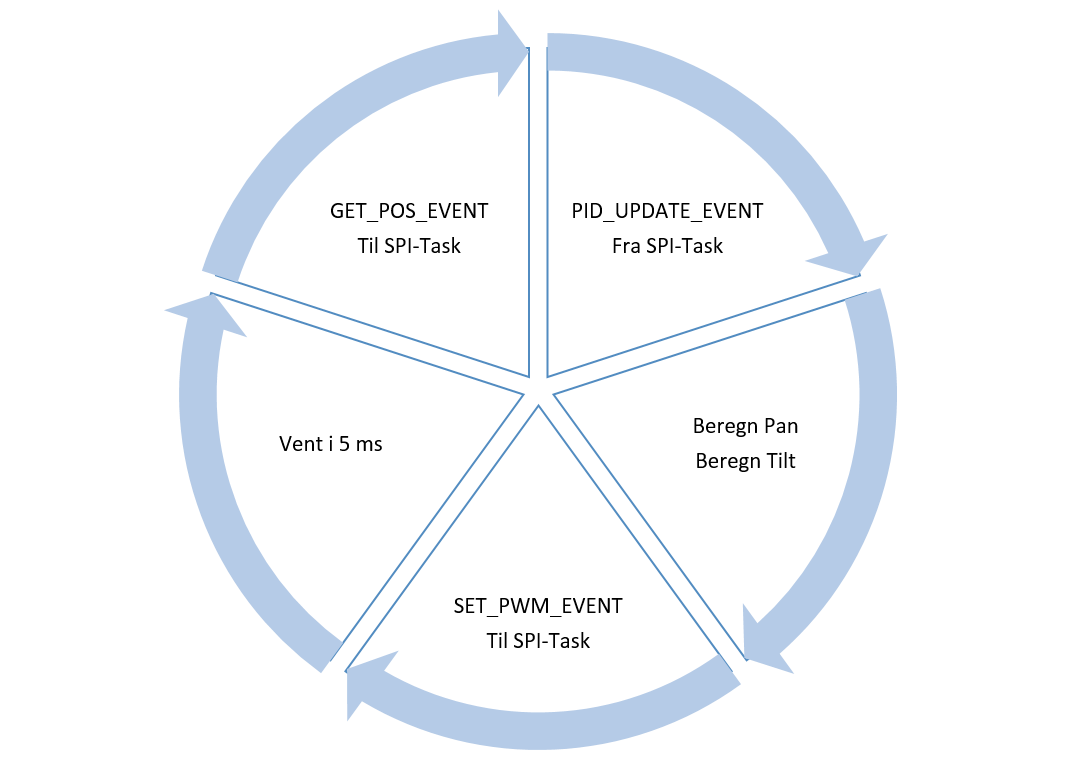
\includegraphics[scale=0.5]{Billeder/PID_update.png}
	\end{center}		
	\caption{Her ses en visualisering af den cyklus som PID-task'en styrer, når den er i running-tilstanden}
	\label{fig:PID_update}
\end{figure}

\paragraph{Filter}
En alternativ måde at gribe implementeringen an på, er at lave controlleren som et filter. Det kan lade sig gøre ved at mappe overføringsfunktionen over i z-domænet og den vej igennem finde filterkoefficienterne. Denne metodik tillader implementeringen af andre controller-typer som fx lead- og lag-controllere, da lettere man kan implementerer flere slags overføringsfunktioner.

\subsubsection{Delkonklusion}

PID-controllleren blev implementeret med en sample frekvens på 200 Hz. Dette afspejler ikke helt præcist den modellerede controller, men det er tæt nok på til at kunne opfylde kravene til projektet. Der kunne også have været brugt \textit{fixed point} aritmetik til udregningerne på microcontrolleren, men det blev vurderet at det skabte flere problemer end det løste under udviklingen. Det er noget som kunne tages op igen på et senere tidspunkt. For at slippe af med integral windup blev der sat et loft på hvor stort integralet kunne blive, og det blev slet ikke brugt, når fejlen var over en bestemt størrelse. For at forhindre oscillationer omkring set point låses motoren når fejlen er 0. En filterimplementering blev ikke udforsket, men kunne helt klart være en mulig forbedring af systemet i fremtiden.

\subsection{Løse funktionaliteter}

\subsubsection{Koordinat oversættelse}

\label{subsec:koordinat}

Da pan og tilt rammen har en præcision på en tredjedel grad, og det samtidigt er et primært krav at denne skal kunne fungerer med input i form af spheriske koordinater, er det nødvendigt at have en koordinat oversættelse fra de inputtede koordinater som er i horizontale koordinater, se figur \ref{fig:Horizontal}. Denne oversættelse skal nødvendigvis tage højde for at de fysiske begrændsninger systemet har. Oversættelsen skal derfor lave en oversættelse i pan delen der afspejler at denne kun kan bevæge sig lidt over 180 grader uden at der opstår problemer med de ledninger der styrer tilt delen. Dette er dog slet ikke nok til at lave et effektivt teleskop system.
\begin{figure}[!h]
	\begin{center}
		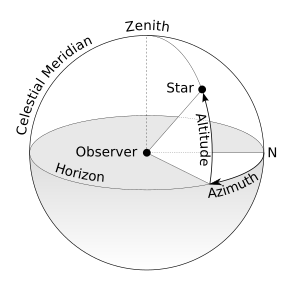
\includegraphics[width=0.5\textwidth]{Billeder/Horizontal.png}
	\end{center}		
	\caption{Her ses hvordan det horizontale koordinat system fungerer}
	\label{fig:Horizontal}
\end{figure}

Mens pan delen kun har 180 graders frihed har tilt delen fuld frihed. Dette betyder at vi kan udnytte denne til at tilgås det område som pan delen ikke kan tilgå. Dette gøres ved blot at spejle tilt delen omkring origo hvis denne skal pege over i dette område, hvilket kan ses i praksis ved at figur \ref{fig:tilt_spejl} er den spejlede version af figur \ref{fig:tilt_spejl1}. Nulpunktet for pan og tilt systemet er lokeret som på figur \ref{fig:Nulpunkt}. 

\begin{figure}[!h]
    \centering
    \begin{subfigure}[b]{0.3\textwidth}
       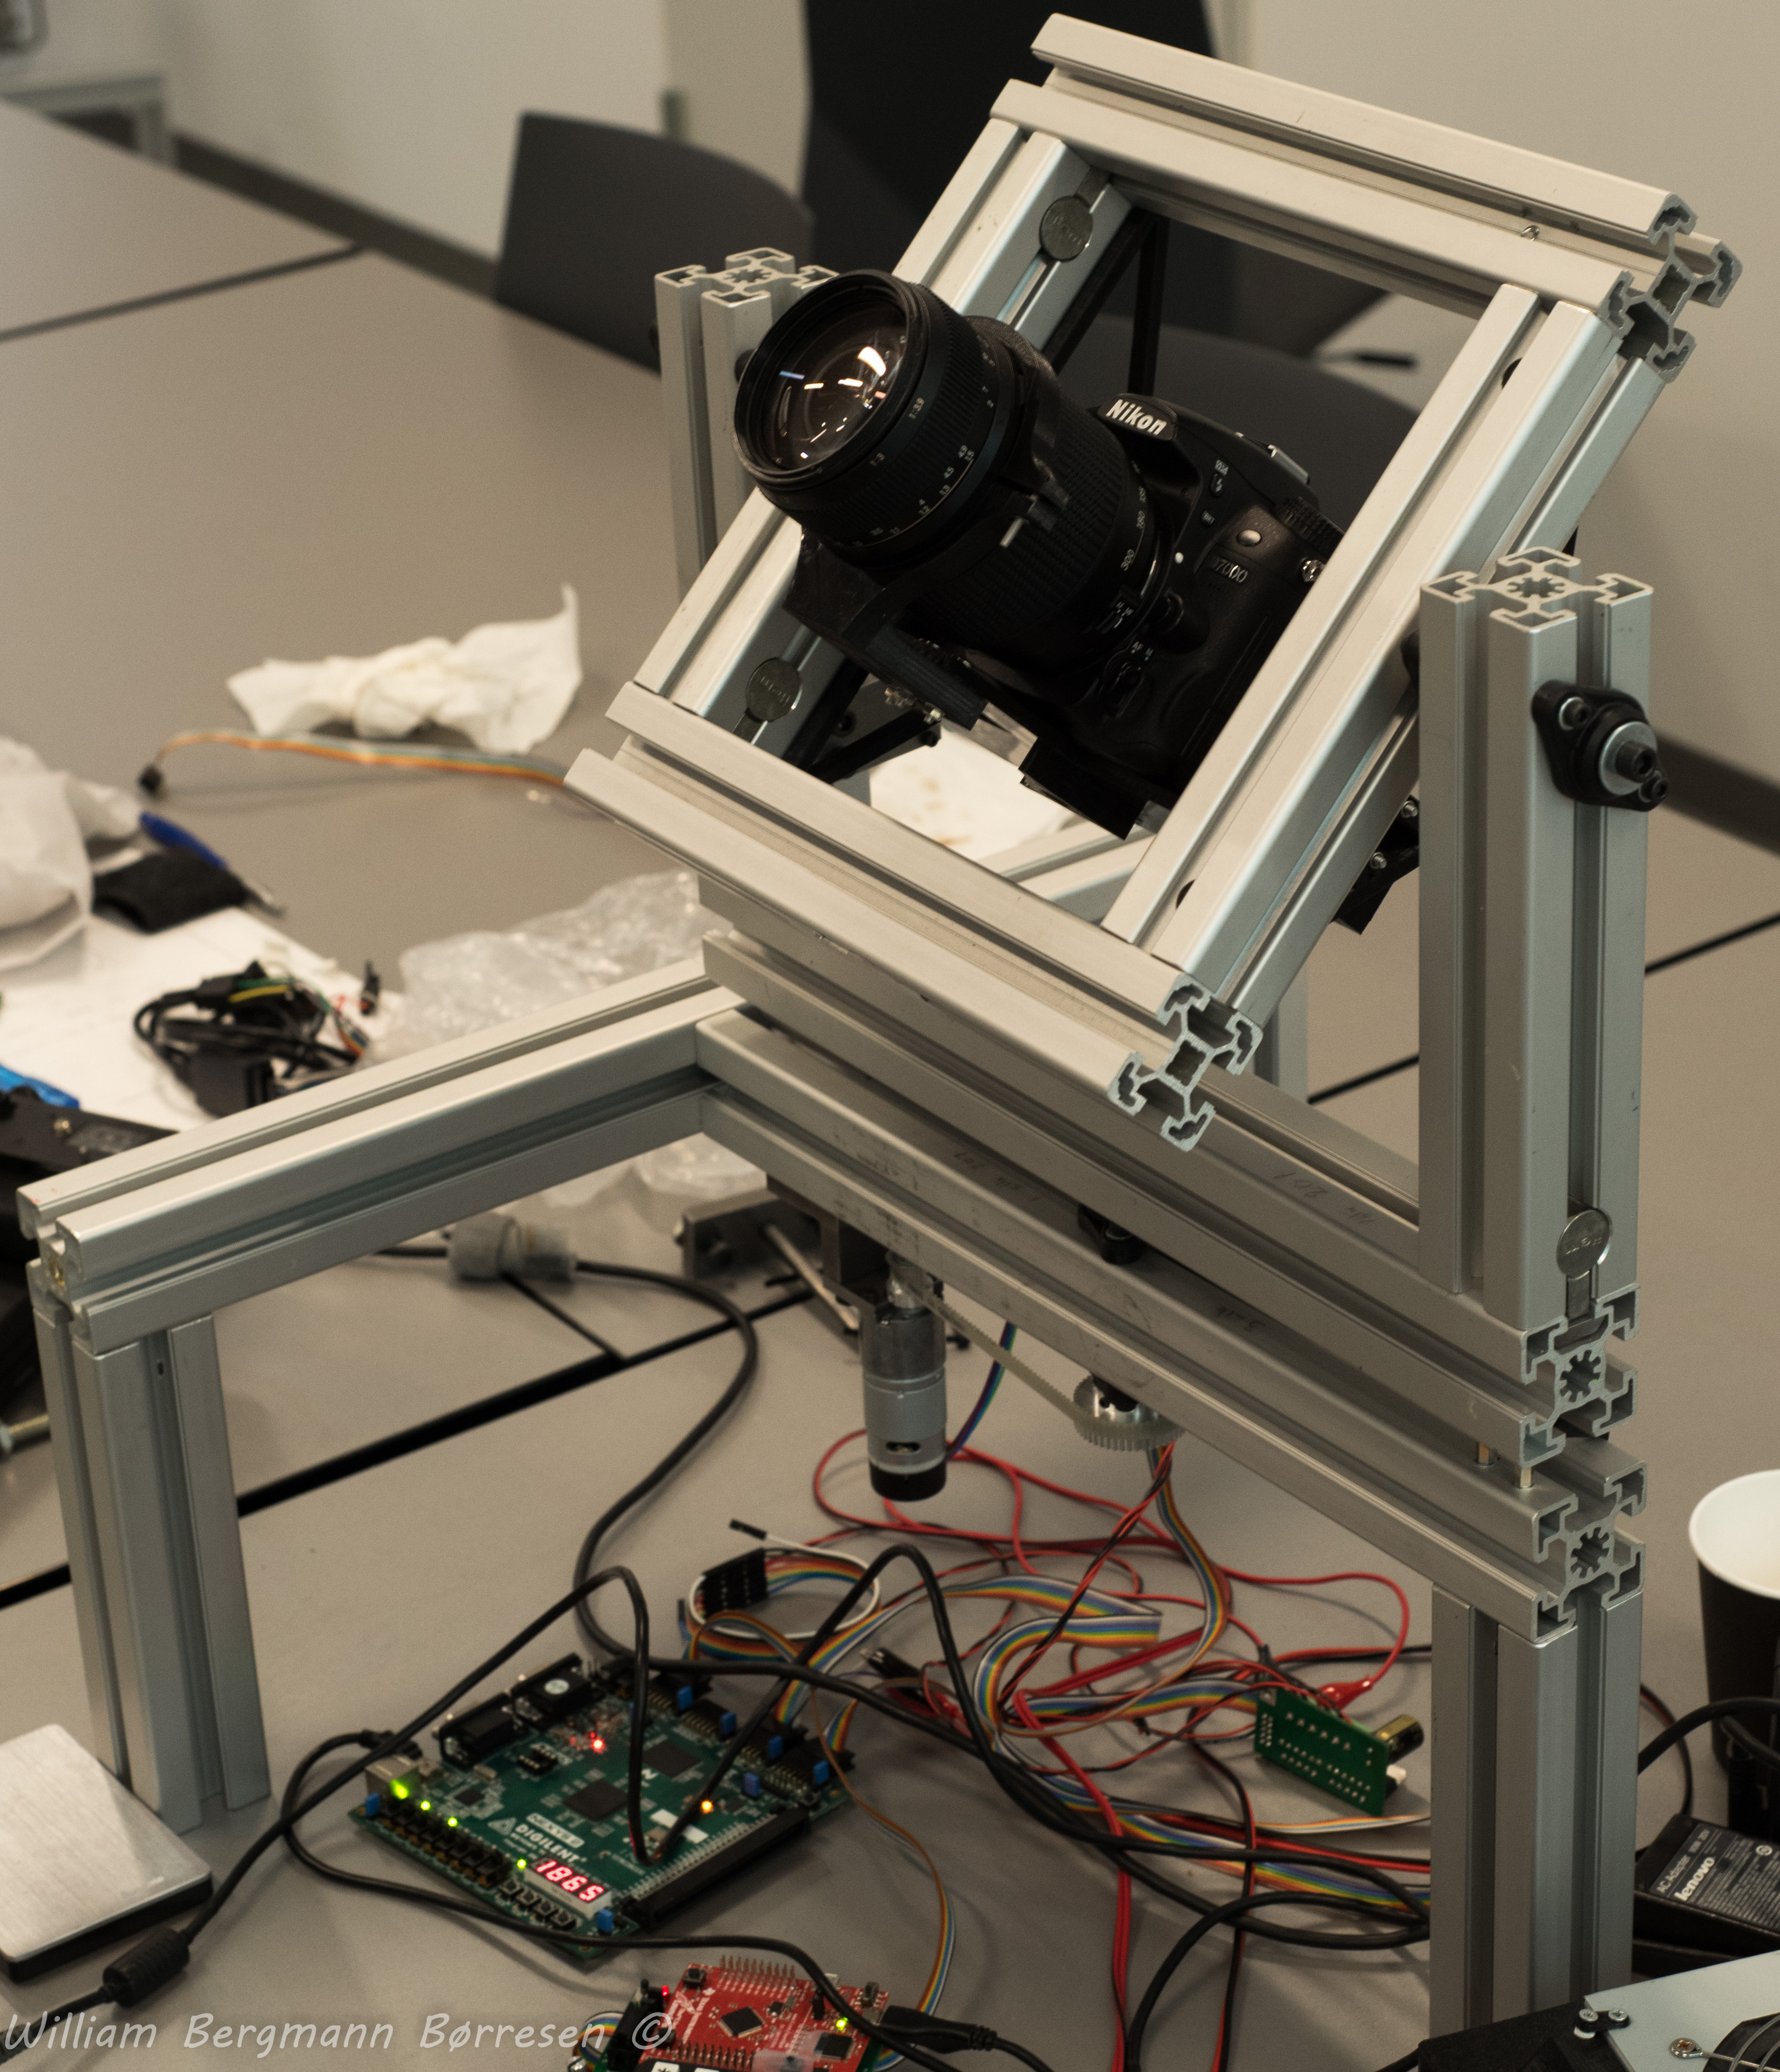
\includegraphics[width=1\textwidth]{Billeder/Tilt45deg.jpg}
        \caption{}
        \label{fig:tilt_spejl1}
    \end{subfigure}
  \begin{subfigure}[b]{0.3\textwidth}
        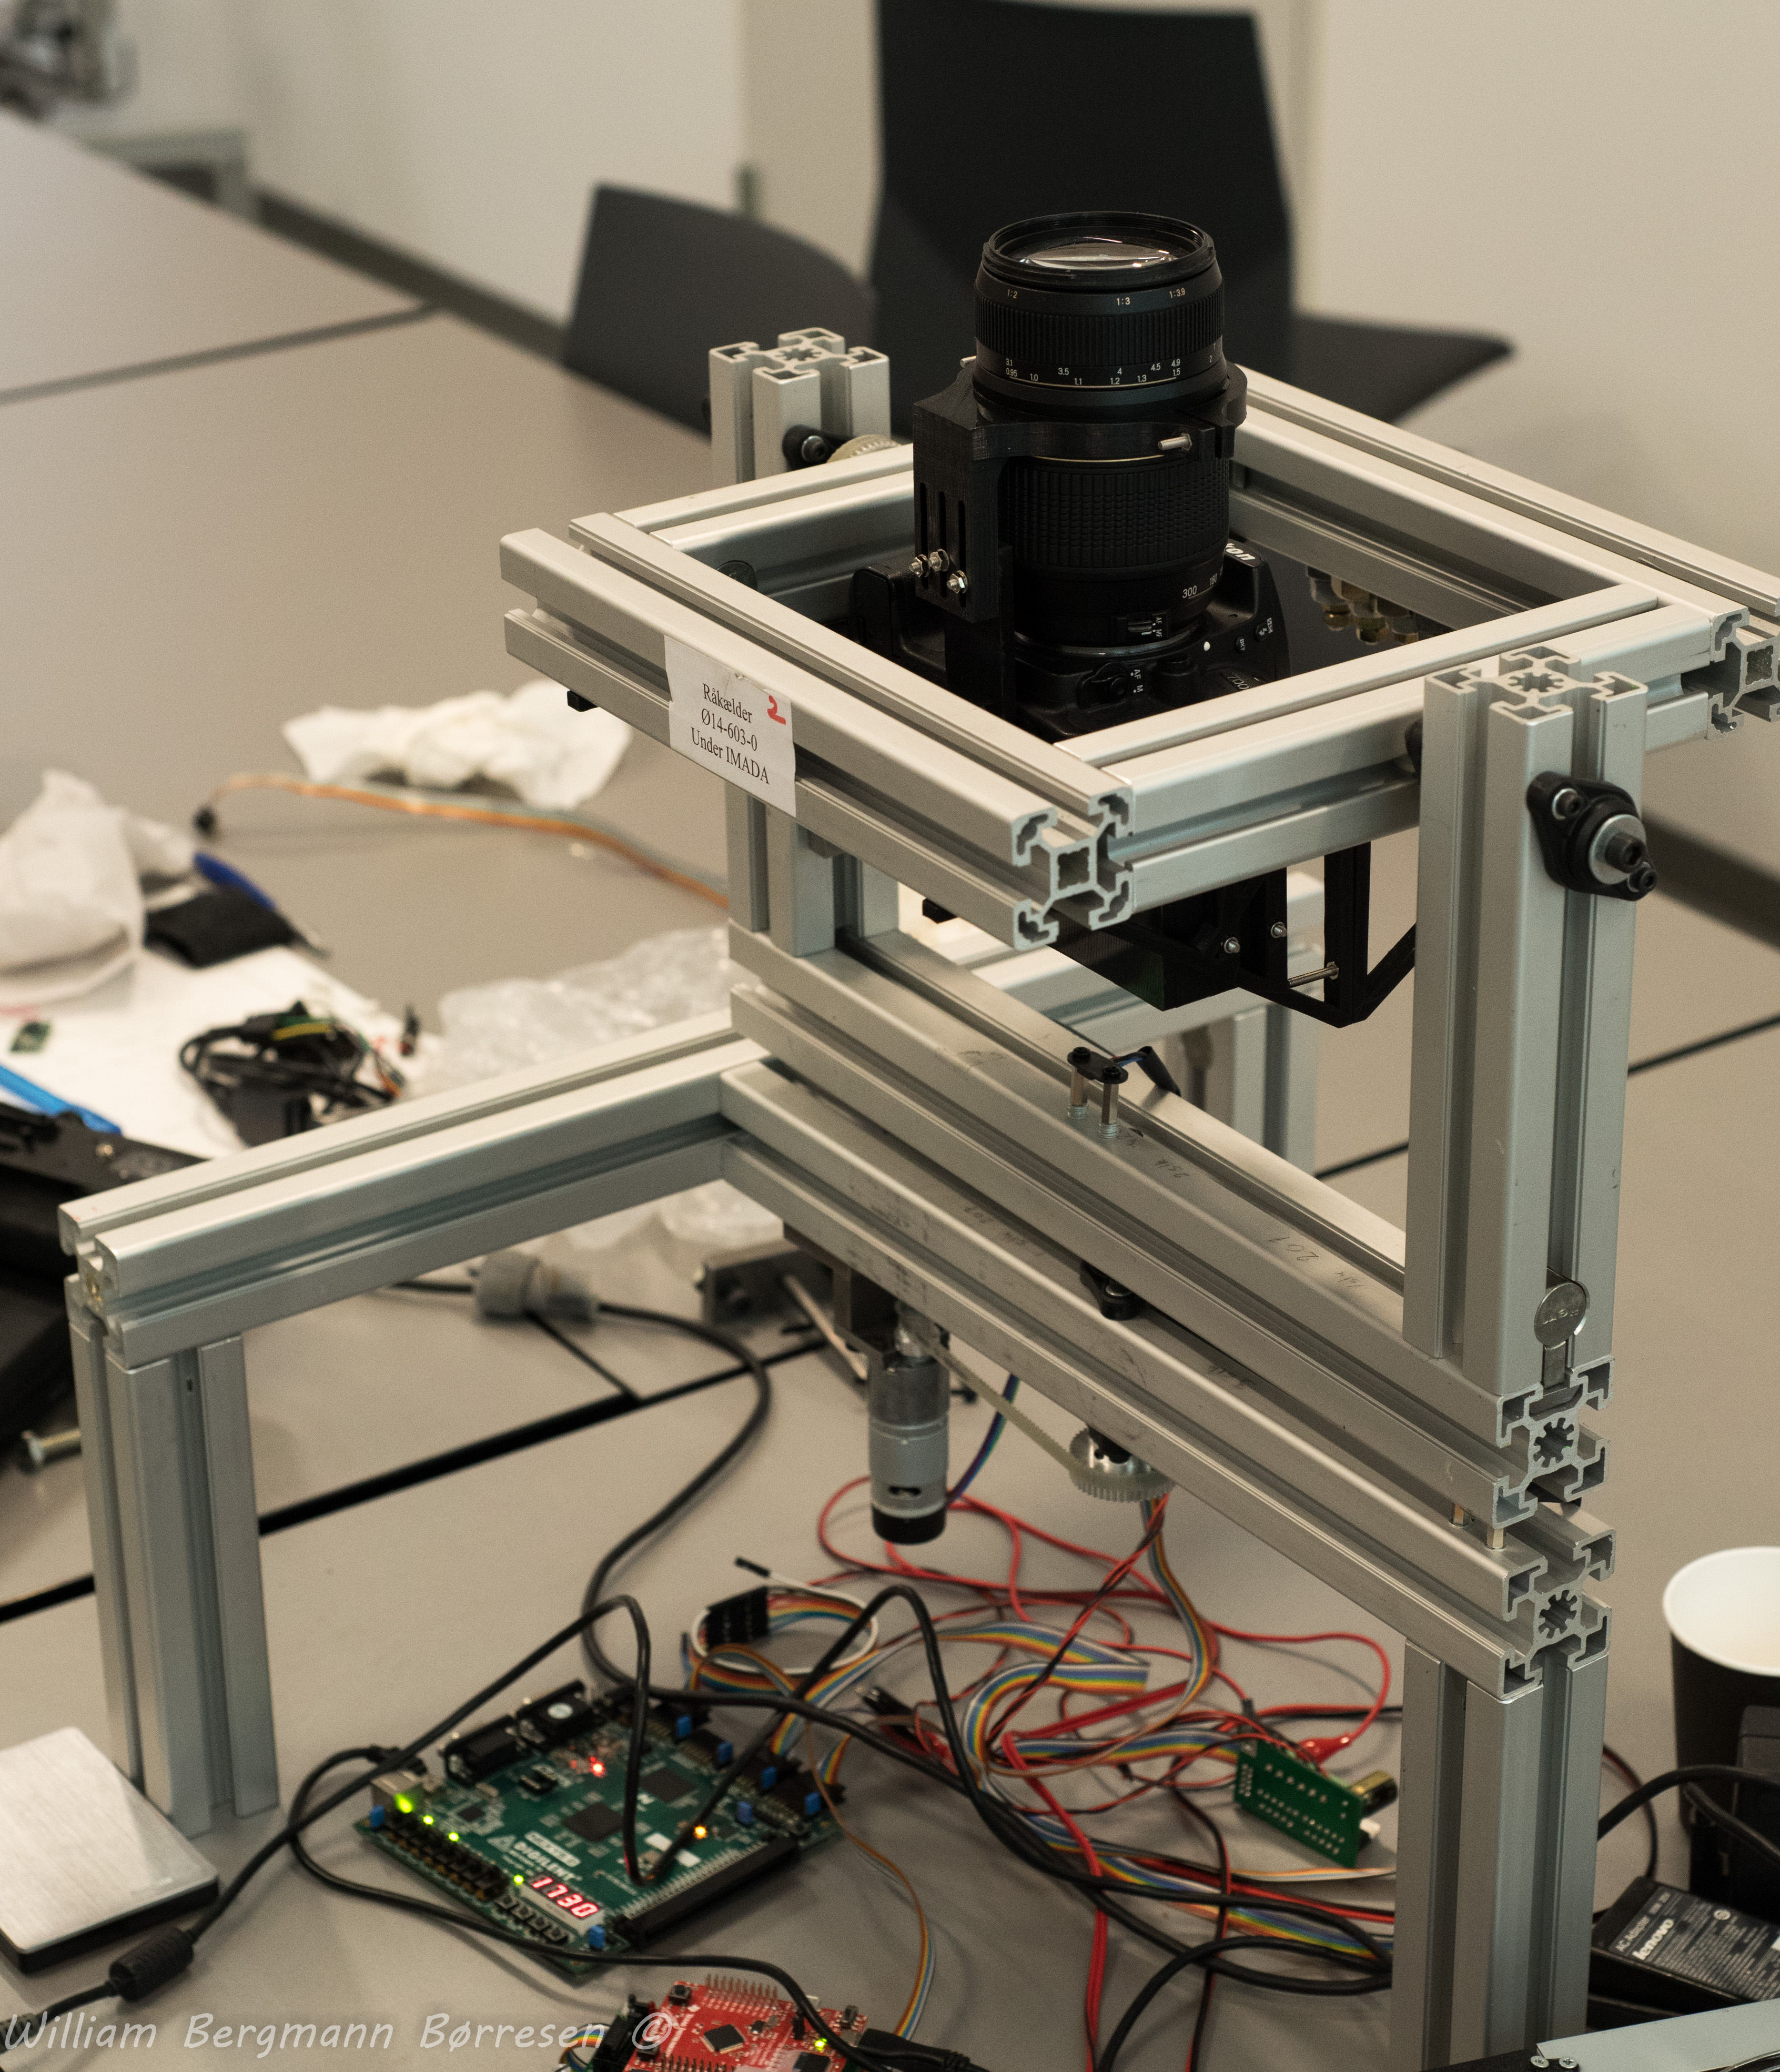
\includegraphics[width=1\textwidth]{Billeder/Nulpunkt.jpg}
        \caption{}
        \label{fig:Nulpunkt}
    \end{subfigure}
    \begin{subfigure}[b]{0.3\textwidth}
        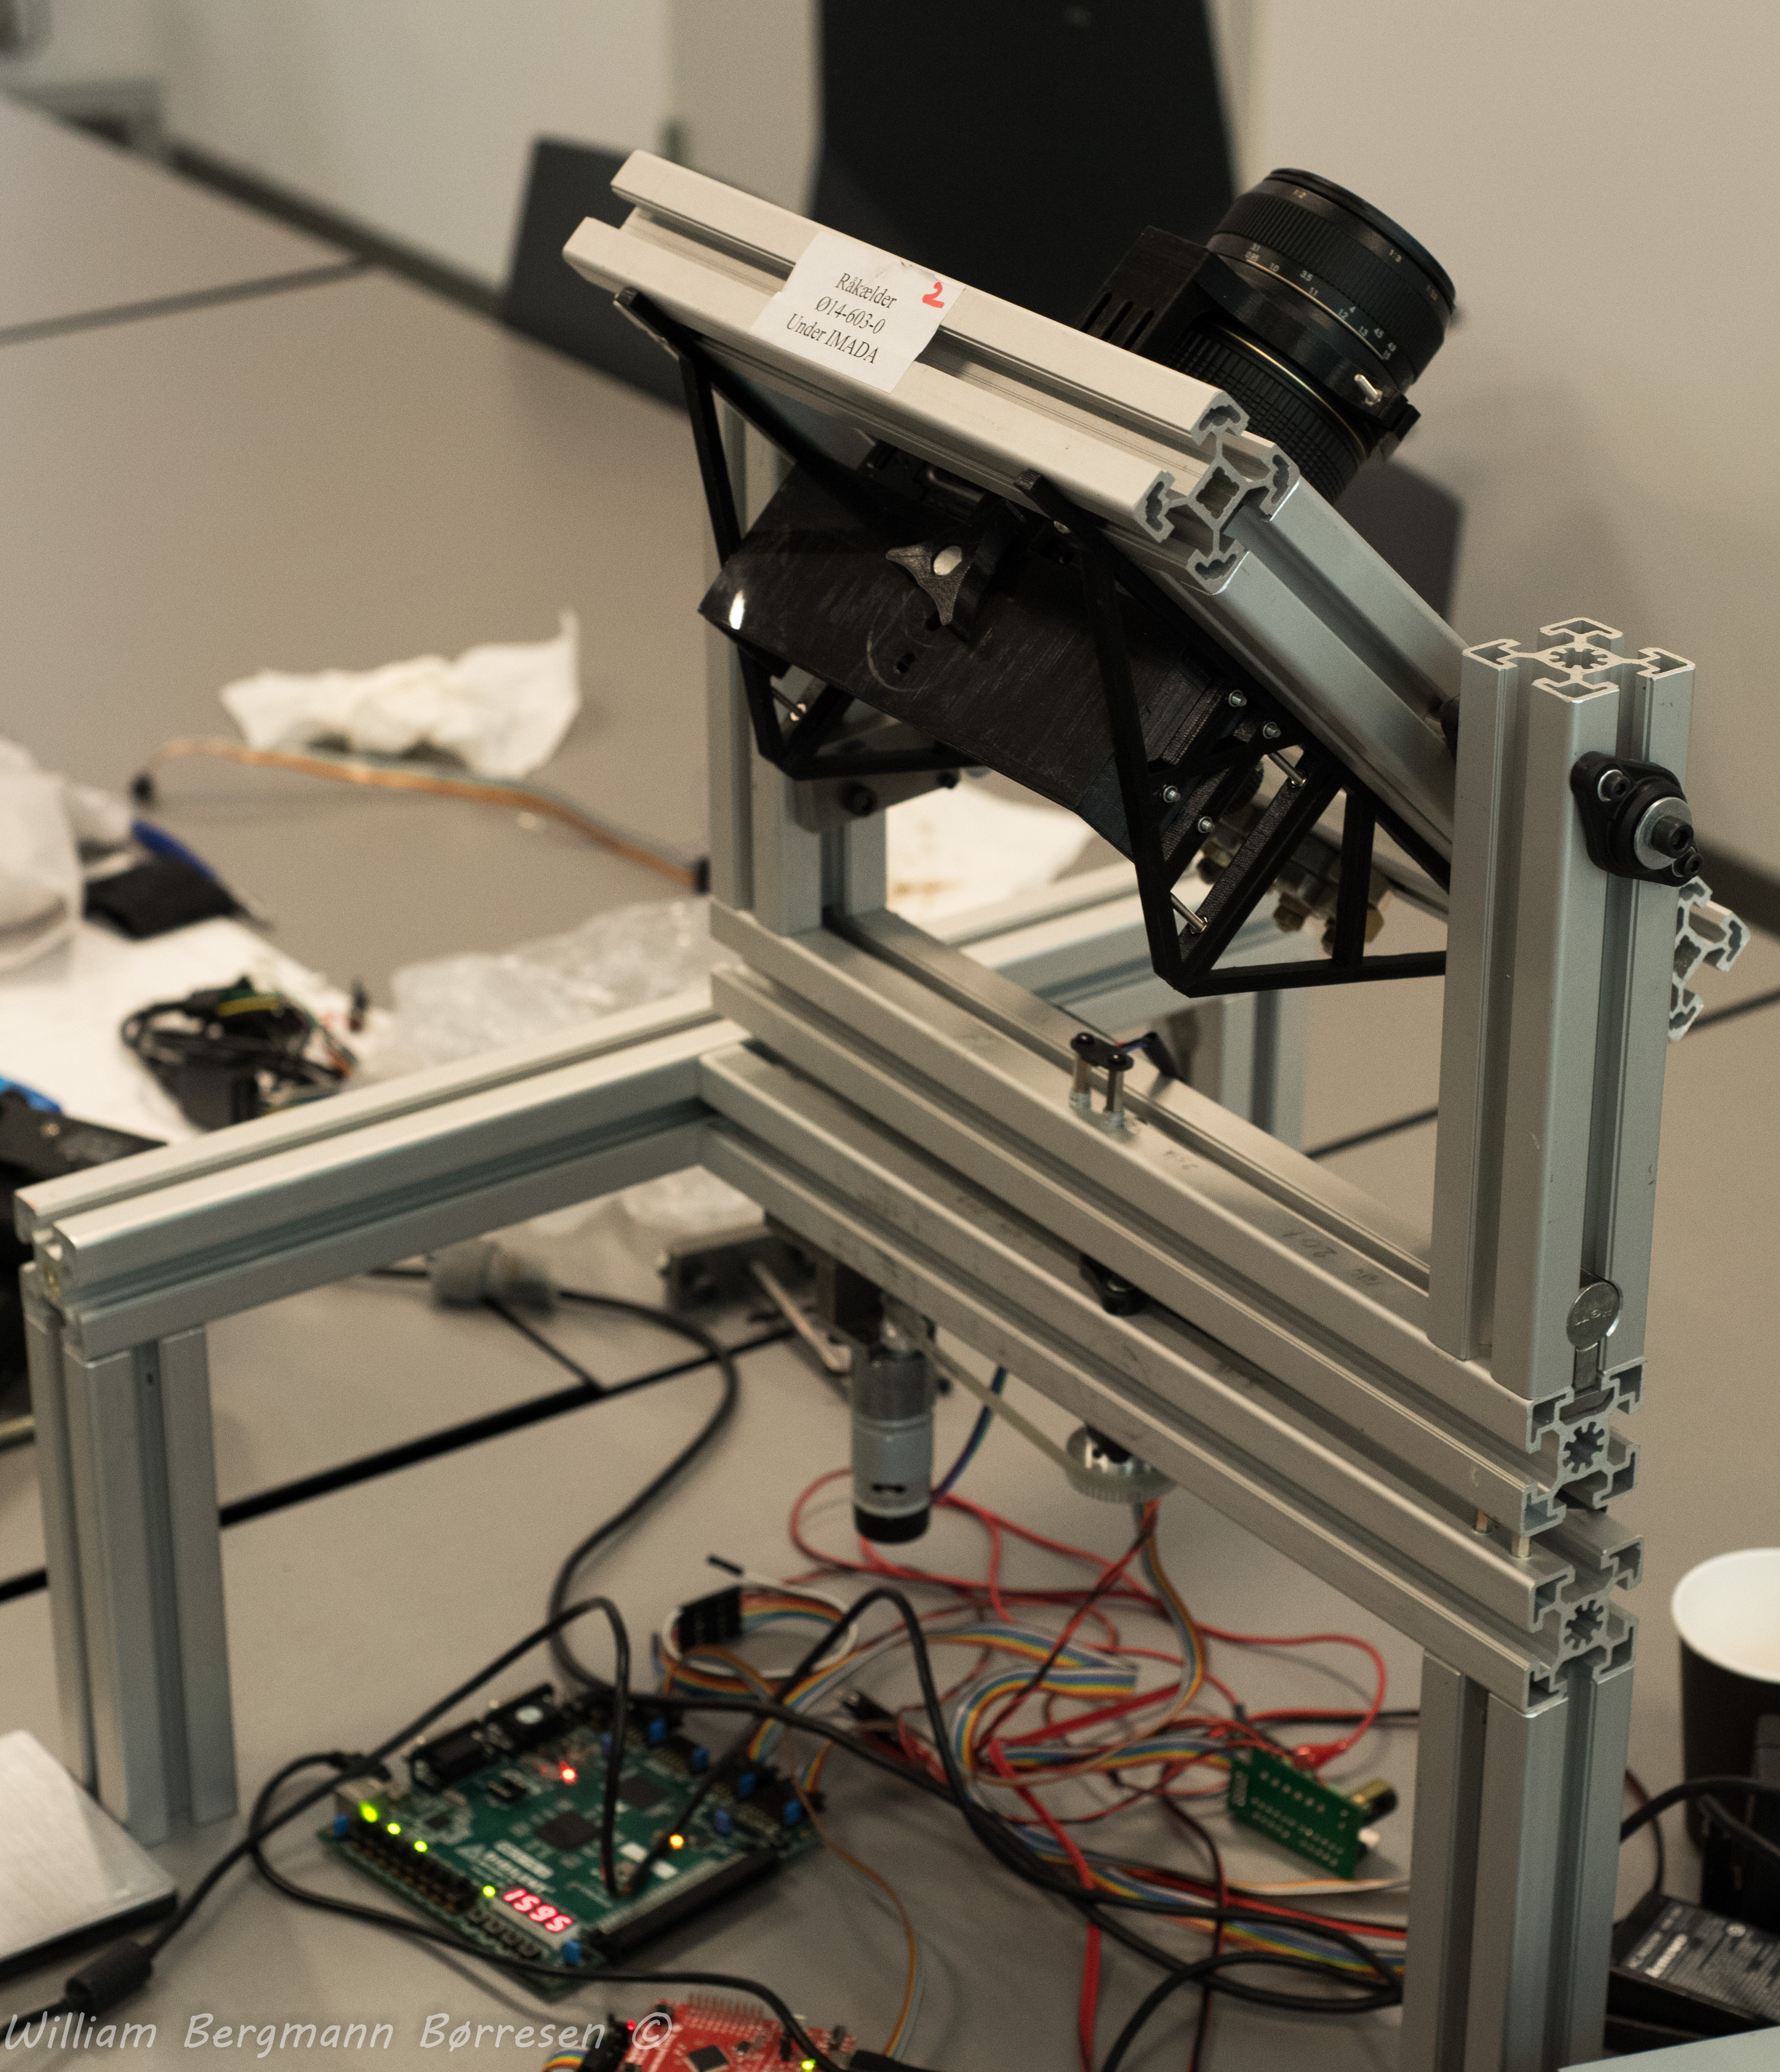
\includegraphics[width=1\textwidth]{Billeder/Tilt315deg.jpg}
        \caption{}
        \label{fig:tilt_spejl}
    \end{subfigure}
   \caption{Her demonstreres hvordan en spejling foregår. Til venstre ses systemet i position pan: 0$^{\circ}$ tilt: 45$^{\circ}$, i midten ses origo ved pan: 0$^{\circ}$, tilt: 0$^{\circ}$, og til højre ses hvad der sker når vi forsøger at bevæge systemet over i det område som pan systemet ikke kan komme over i, ved pan: 180$^{\circ}$, tilt: 45$^{\circ}$.}
\end{figure}

Denne position er valgt fordi den passer bedst overens med det spheriske koordinat system, som kan ses på figur \ref{fig:Spherical}. Alternativt kunne det pladseres således at pan delen havde sigt nulpunkt i kanten  af dens bevægelsesområde, men dette blev fravalgt da den sensor der benyttes til at indstille systemet ligger på denne position. Grunden til at dette ikke er gjort for tilt systemet er at denne retning både gør det nemmere at spejle det omkring origo, samt at det passer bedre med vores spheriske koordinat system.
%Løsningen til dette er at tilt delen bliver spejlet omkring origo når systemet forsøger at pege mod et punkt der ligger i området mellem 90 og 270 grader i forhold til det valgte nulpunkt ved hall sensoren. Grunden til at systemet kan bevæge sig 90 grader til hver side, omend dette kan virke irrationelt, er at dette er positionen af den hall sensor der benyttes til at nulstille koordinat systemet på FPGA'en. Nulpunktet i tilt delen af teleskop systemet er positioneret direkte opad, da dette både gjorde det mindre kompliceret at spejle det, og samtidig passede bedre overens med det polære koordinat system. Der kunne argumenteres for at det ville være nemmere også at sætte dennes nulpunkt der hvor hall sensoren nulstiller FPGA'en, men dette blev valgt fordi det er mere modulært at gå efter et system der mere matematisk intuitivt.

\begin{figure}[!ht]
	\begin{center}
		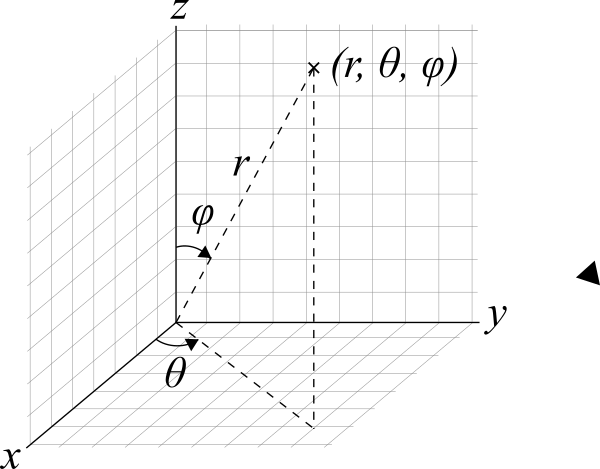
\includegraphics[width=0.5\textwidth]{Billeder/Spherical.png}
	\end{center}		
	\caption{Her ses hvordan det valgte spheriske koordinat system fungerer. Der er flere mulige baser for spheriske koordinater, men dette er det mest matematisk rigtige, hvilket er grundet til at dette blev valgt.}
	\label{fig:Spherical}
\end{figure}

En stor fordel ved denne koordinat oversættelse er at den eliminerer nødvendigheden for et sikkerhedssystem på microcontrolleren. Dette er naturligt en del af koordinat oversættelsen, da alt mellem 90 og 270 grader på pan systemet, som er de områder hvor der kan ske mekaniske skader, slet ikke er aktuelt, på grund af spejlingen af koordinaterne. Det skal dog noteres at dette ikke eliminerer behovet for et sikkerhedssystem på FPGA'en, som der stadig er brug for i tilfælde af et der forekommer problemer med microcontrolleren, så som en løs forbindelse, en fejl der får hele microprocessoren til at fryse, eller overshoot der går ud over den sikkerheds grænse der er blevet besluttet.




















